% Estado del arte
\chapter{Estado del arte} \label{ch:estado}
    En este capítulo se van a presentar distintas tecnologías de virtualización, aprovisionamiento y despliegue aplicables al proyecto. Estas tecnologías se analizan y comparan para posteriormente seleccionar aquellas que mejor se adecuen a los objetivos que se pretenden conseguir.

\section{Tecnologías de virtualización} \label{sec:virt}
	Se podría decir que la virtualización es ya uno de los pilares fundamentales del mundo IT debido a las grandes ventajas que proporciona. Previo al desarrollo de las tecnologías y tipos de virtualización disponibles, es conveniente explicar en qué consiste la virtualización, que no es más que una representación mediante software de un entorno físico o recurso tecnológico, como pueden ser aplicaciones, servidores o almacenamiento.~\cite{virt1} 

	Gracias a esta tecnología, es posible contar con varios ordenadores virtuales en el mismo hardware, donde cada uno de ellos puede interactuar de forma independiente y ejecutar sistemas operativos o aplicaciones diferentes mientras comparten los recursos de una sola máquina host. Al crear varios recursos a partir de un único equipo o servidor, la virtualización mejora la escalabilidad y las cargas de trabajo, al tiempo que permite usar menos servidores y reducir el consumo de energía, los costos de infraestructura y el mantenimiento.

	En función del sistema a simular, podemos encontrar diferentes categorías~\cite{virt2}, un ejemplo es la virtualización de red, que consiste en crear redes virtuales sobre redes físicas o reproducir completamente redes físicas en software. Otro ejemplo sería la virtualización de almacenamiento, que combina varios dispositivos de almacenamiento en red, con la apariencia de una única unidad o dispositivo de almacenamiento, accesible por varios usuarios. Podríamos enumerar más tipos de virtualización, pero en lo que a este trabajo respecta vamos a centrarnos en la virtualización de software, que separa las aplicaciones del hardware y el sistema operativo, y en la que distinguimos dos subtipos: virtualización mediante hipervisor y virtualización en contenedores.

\subsection{Virtualización mediante hipervisor} \label{sec:hiperv}
	Una máquina virtual es un software que ejecuta programas o procesos como si fuera la máquina física. Es decir, se abstrae el hardware y se representa con una capa de software que proporciona una interfaz igual que el hardware, de forma que sobre ella podemos instalar uno o varios sistema operativos invitados o \textit{guests} distintos. Esta capa de software también se encarga de repartir y aislar los recursos del host entre las VM, de manera que el host queda protegido si falla una VM, y las VM estén protegidas entre ellas. Pues bien, cuando hablamos de esta capa de software estamos hablando de lo que se conoce como hipervisor. 

	Como ya se ha mencionado, un hipervisor es una capa intermedia de software que permite al ordenador anfitrión prestar soporte a varias máquinas virtuales mediante el uso compartido de sus recursos. Cuando se ejecuta una instrucción en el OS invitado, el hipervisor la coje y la ejecuta en el OS anfitrión. En este proceso, el OS no diferencia entre ejecutar procesos en la máquina virtual o en la física, lo que representa plenamente el concepto de virtualización.

	Dentro de los hipervisores~\cite{virt3}, podemos distinguir dos tipos. El primero es el Tipo 1, conocido también como hipervisor nativo o \textit{bare-metal}. Este hipervisor se ejecuta directamente sobre el hardware en lugar de un OS clásico. Todos los hipervisores necesitan algunos elementos del sistema operativo (por ejemplo, el administrador de memoria, el programador de procesos, la pila de entrada o salida [E/S], los controladores de dispositivos, entre otros) para ejecutar las máquinas virtuales. Por tanto, este hipervisor es equivalente a un OS con un poco de información adicional que le permite gestionar los OS invitados. Es muy común encontrarlos en centros de datos, por la eficiencia que supone el ahorrar una capa de software.

	Los hipervisores de Tipo 2 se ejecutan sobre el OS anfitrión como una capa de software o aplicación. Están orientados a usuarios individuales que buscan ejecutar varios OS en el mismo ordenador. La ejecución de una VM sobre un hipervisor de este tipo es más lenta que en un hipervisor de Tipo 1.

	\begin{figure}[h]
	\centering
	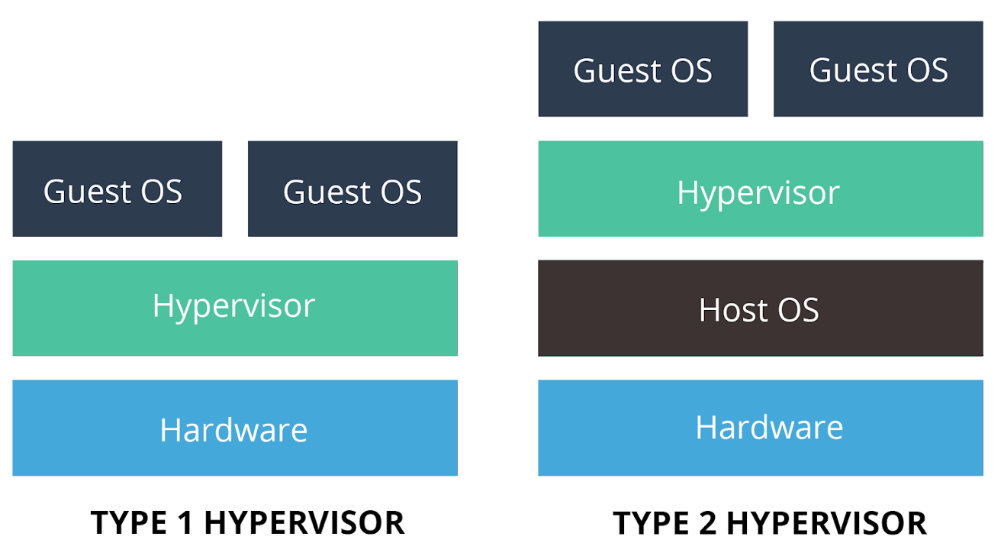
\includegraphics[width=0.7\textwidth]{../imgs/EdA/hipervisor.jpg}
	\caption{Tipos de hipervisor}
	\label{fig:hipervtypes}
	\end{figure}

	A continuación se presentan algunas tecnologías que emplean este tipo de virtualización.
	\clearpage

\subsubsection{KVM}
	KVM (Kernel Virtual Machine)~\cite{kvm} es una tecnología de virtualización open source que convierte el kernel de Linux en un hipervisor de Tipo 1 que se puede usar para la virtualización. Las KVM tienen todos los elementos necesarios de un OS porque forman parte del kernel de Linux. Cada máquina virtual se implementa como un proceso habitual de Linux. Al ser un hipervisor de Tipo 1 ofrece un mejor rendimiento. 

	\begin{figure}[h]
	\centering
	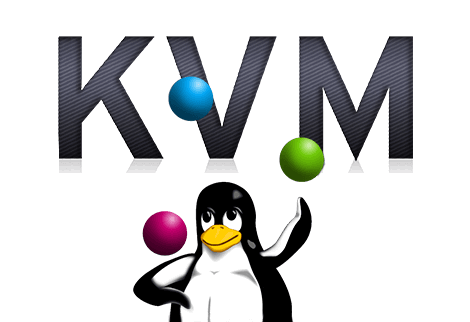
\includegraphics[width=0.3\textwidth]{../imgs/EdA/kvm.png}
	\caption{Logo de KVM}
	\label{fig:kvm}
	\end{figure}

	La configuración de la máquina virtual creada se almacena internamente en un fichero XML, el cual es posible editar manualmente a posteriori si se quiere hacer algún cambio. KVM nos permite disfrutar de las ventajas del software open source: no habrá restricciones en cuanto a integración, como sí puede haberlas si se usa un software propietario como VMware; y es independiente de proveedores. Es posible instalar una GUI como virt-manager, que se apoya en la biblioteca libvirt (API de virtualización estándar de Linux), para facilitar su uso.

\subsubsection{VirtualBox}
	VirtualBox~\cite{vbox} es desarrollado por Oracle, aunque es gratuito y open source al igual que KVM. Es un hipervisor de Tipo 2, por lo que ofrece un rendimiento inferior comparado con un Tipo 1. VirtualBox permite crear y cargar máquinas virtuales de una forma muy sencilla, lo que hace que sea la alternativa elegida por muchos usuarios. Su asistente ofrece algunos valores sugeridos para tipos específicos de máquinas virtuales durante la creación de estas, pero su gestión final se produce en una configuración posterior.

	\begin{figure}[h]
	\centering
	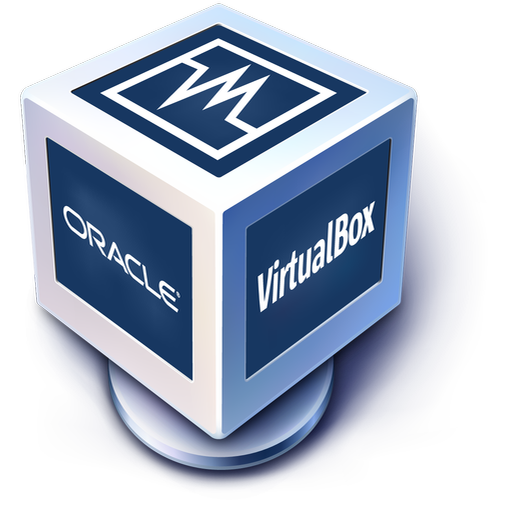
\includegraphics[width=0.2\textwidth]{../imgs/EdA/vbox.png}
	\caption{Logo de VirtualBox}
	\label{fig:vbox}
	\end{figure}

	Una ventaja de VirtualBox son las instantáneas, que permiten tomar una imagen de la máquina virtual en un momento dado. La imagen conserva la máquina virtual, lo que permite volver a ese momento específico.

	VirtualBox ofrece un soporte muy completo. Tiene versiones para Windows, Linux, Macintosh y Solaris, y puede ejecutar un amplísimo número de sistemas operativos invitados, incluidos Windows, macOS, Linux, DOS, Solaris u OpenBSD.

\subsubsection{VMware}
	VMware~\cite{vmware} es un software comercial, lo que significa que si queremos aprovechar al máximo todas sus herramientas y configuraciones, debemos pagar por la licencia de uso. Aquí vamos a hablar de VMware Workstation Player, que es el producto gratuito de VMware para virtualización de máquinas, orientado para uso personal, doméstico y sistema educativo. 

	\begin{figure}[h]
	\centering
	
\includegraphics[width=0.2\textwidth]{../imgs/EdA/vmware.png}
	\caption{Logo de VMware}
	\label{fig:vmware}
	\end{figure}

	En comparación con VirtualBox, VMware Workstation Player es una experiencia más fluida y ágil, y ofrece mejor soporte y estabilidad para una amplia gama de hardware. Está disponible para Windows y Linux y también admite todo tipo de sistemas invitados.~\cite{versus}

	Además, VMware Workstation Player sí permite personalizar toda la configuración durante el proceso de creación de la máquina virtual. La diferencia no es mucha, pero significa que la máquina virtual está lista para ejecutarse después de finalizar el asistente, en lugar de tener que realizar más configuraciones una vez que se completa.

	Por el contrario, no admite instantáneas o puntos de control. Puede suspender temporalmente el sistema operativo invitado para reanudar desde un punto específico, pero no es tan completo como la creación de un historial de imágenes para la máquina virtual.

	\clearpage

\subsection{Virtualización en contenedores} \label{sec:cont}
	La virtualización basada en contenedores, también llamada virtualización del sistema operativo, es una aproximación a la virtualización en la cual la capa de virtualización se ejecuta como una aplicación en el sistema operativo.

	Un contenedor~\cite{cont1} es un conjunto de uno o más procesos aislados del resto del sistema, que acceden sólo a los recursos que se indican. El contenedor encapsula el programa específico y las librerías, mientras que utiliza el sistema operativo del host. Podemos distinguir entre dos tipos de contenedores:~\cite{cont2}

	\begin{itemize}
		\item \textbf{A nivel de sistema operativo:} un sistema operativo completo se ejecuta en un espacio aislado dentro de la máquina host, compartiendo el mismo kernel.
		\item \textbf{A nivel de aplicación:} una aplicación o servicio, y los procesos mínimos requeridos por esa aplicación, se ejecutan en un espacio aislado dentro de la máquina host.
	\end{itemize}

	Al compartir el mismo kernel del sistema operativo host, un contenedor sólo puede ejecutar procesos en ese sistema operativo. Es decir, un contenedor que se ejecuta en un servidor de Linux, por ejemplo, solo puede ejecutar un sistema operativo Linux, mientras que tal y como habíamos comentado, un hipervisor emula el hardware, lo que permite que varios sistemas operativos (Windows o Linux) se ejecuten simultáneamente en un solo sistema. Además, esta compartición del núcleo hace que el nivel de aislamiento sea menor comparado con las máquinas virtuales, ya que al acceder todos los contenedores al mismo núcleo, si se explota una vulnerabilidad en el núcleo ésta afectaría a todo el sistema, incluidos todos los contenedores.

	A cambio, con la virtualización basada en contenedores, no existe la sobrecarga asociada con tener a cada huésped ejecutando un sistema operativo completamente instalado. Este enfoque también puede mejorar el rendimiento porque hay un solo sistema operativo encargándose de los avisos de hardware.

	Tal y como se ha mencionado previamente, los contenedores hacen uso del kernel del sistema operativo, del que cabe destacar las siguientes características necesarias para el correcto funcionamiento de este tipo de virtualización:~\cite{cont3}

	\begin{itemize}
		\item \textbf{Grupos de control o cgroups.} Se encargan de gestionar los recursos del ordenador asignados a un proceso o conjunto de procesos, como pueden ser el número de \textit{slices} de tiempo de CPU asignadas a cada proceso, el límite de memoria a usar por proceso, los dispositivos de bloques de E/S… Es posible estructurar los recursos en jerarquía.
		\item \textbf{Namespaces.} Permiten aislar procesos entre sí. Los procesos de un contenedor se asignan a un namespace, y el sistema operativo aísla los recursos entre ese namespace y el resto. Hay diferentes tipos de namespace: de PID, que permiten mantener los mismos PIDs en diferentes contenedores; mount, para separar sistemas de ficheros; de red para aislar controladores de red… 
	\end{itemize}

	Los contenedores, por tanto, suponen una virtualización más ligera: usan menos recursos que las máquinas virtuales, además de proporcionar mayor flexibilidad y rapidez de arranque y despliegue. Esto último se debe a que, al usar el mismo kernel que el host, sólo están iniciando procesos, algo que es casi instantáneo y que hace muy fluida la ejecución de diferentes máquinas a la vez.

	Para contextualizar con el apartado \ref{sec:hiperv}, se muestra una imagen comparativa de la estructura de un contenedor respecto a una máquina virtual:

	\begin{figure}[h]
	\centering
	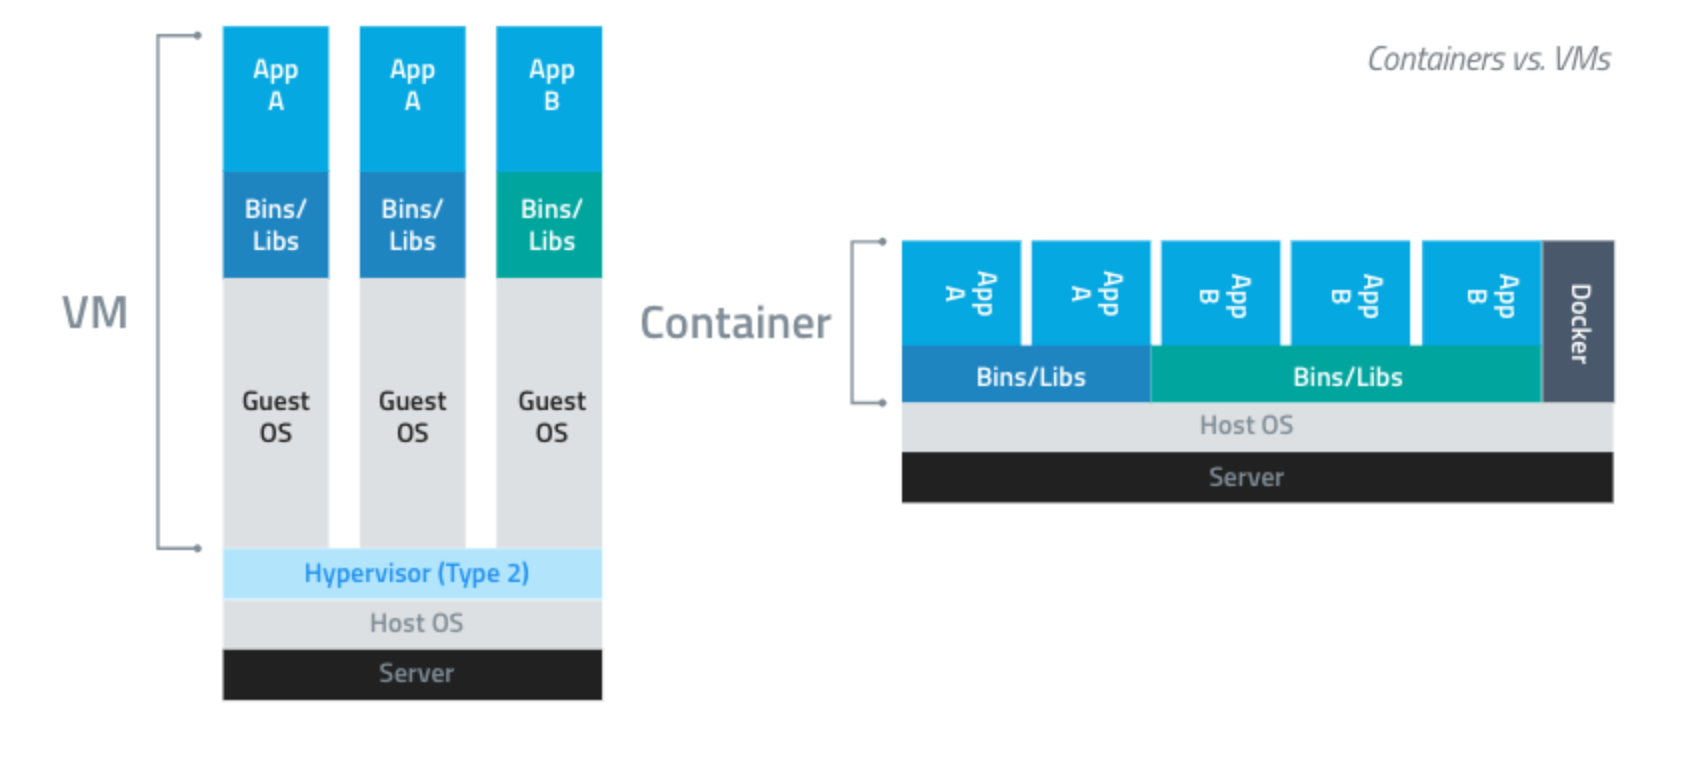
\includegraphics[width=\textwidth]{../imgs/EdA/VMvsCont.png}
	\caption{Contenedor vs VM: Estructura}
	\label{fig:VMvsDocker}
	\end{figure}

\subsubsection{LXC}
	LXC (Linux Containers)~\cite{lxc} es una plataforma de código abierto de contenedores a nivel de sistema operativo. Este tipo de contenedores hacen que un único host Linux actúe como varios host Linux. Esto es debido a que los contenedores LXC incluyen un sistema Linux prácticamente completo, similar a una VM, con su propio sistema de ficheros, espacio de red y aplicaciones. Su objetivo es recrear un entorno lo más parecido posible a una instalación de Linux, pero sin la necesidad de un kernel independiente. 

	\begin{figure}[h]
	\centering
	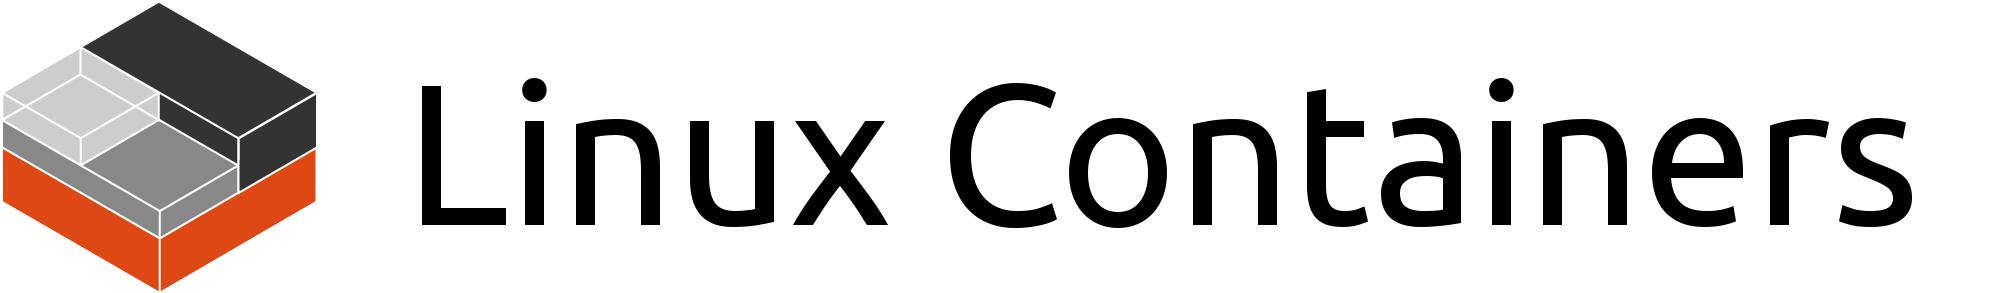
\includegraphics[width=0.5\textwidth]{../imgs/EdA/lxc.png}
	\caption{Logo de LXC}
	\label{fig:lxc}
	\end{figure}

	Chroot es un comando UNIX que permite ejecutar un proceso bajo un directorio raíz simulado, de manera que el proceso no puede acceder a archivos fuera de ese directorio. LXC es similar a un chroot, pero ofrece mucho más aislamiento. 

	Para crear diferentes contenedores de sistema operativo, se emplean plantillas o templates. Las plantillas proporcionadas en LXC son scripts específicos de un sistema operativo.

	LXC se suele usar junto a LXD. LXD ofrece una interfaz para gestionar contenedores LXC como si fueran máquinas virtuales, proporcionando snapshots y control de imágenes, además de otras funcionalidades que incrementan el potencial de LXC. Una de las ventajas principales de LXC es que es una tecnología sencilla de manejar.
\clearpage

\subsubsection{Docker}
	Docker~\cite{docker1} es uno de los proyectos más conocidos y utilizados en este tipo de virtualización. Lejos de ser un sistema operativo como tal, esta plataforma de código abierto hace uso de las funciones de aislamiento de recursos del kernel de Linux para dar lugar a contenedores independientes. Está basada en Linux, pero en los últimos años se ha producido un desarrollo y actualmente también es posible su uso en Windows.

	Los contenedores que proporciona Docker son a nivel de aplicación (puede ejecutar aplicaciones normales sin incluir un sistema operativo completo), y su implementación está basada en imágenes, lo que permite compartir una aplicación o un conjunto de servicios, con todas sus dependencias, en varios entornos.

	Docker utiliza una arquitectura cliente-servidor. En este tipo de arquitectura, las tareas se reparten entre los proveedores de recursos o servicios, llamados servidores, y quienes demandan esos recursos o servicios, que son los clientes. Un sistema de contenedores Docker se compone principalmente de 5 elementos:~\cite{docker2}

	\begin{itemize}
		\item \textbf{Demonio:} es el proceso principal de la plataforma.
		\item \textbf{Cliente:} binario que constituye la interfaz y que permite al usuario interactuar con el Demonio mediante CLI.
		\item \textbf{Imagen:} plantilla utilizada para crear el contenedor para la aplicación que queremos ejecutar.
		\item \textbf{Registros:} directorios donde se almacenan las imágenes, tanto de acceso público como privado. El más común es Docker Hub.
		\item \textbf{Contenedores:} carpetas donde se almacena todo lo necesario (librerías, dependencias, binarios, etc) para que la aplicación pueda ejecutarse de forma aislada.
	\end{itemize}

	Docker Engine es la aplicación cliente-servidor responsable de iniciar y parar los contenidos de una manera similar a como lo hace el hipervisor en una máquina virtual. A continuación se muestra una figura donde se muestran de forma gráfica las interacciones entre los ya mencionados componentes:
	\begin{figure}[h]
	\centering
	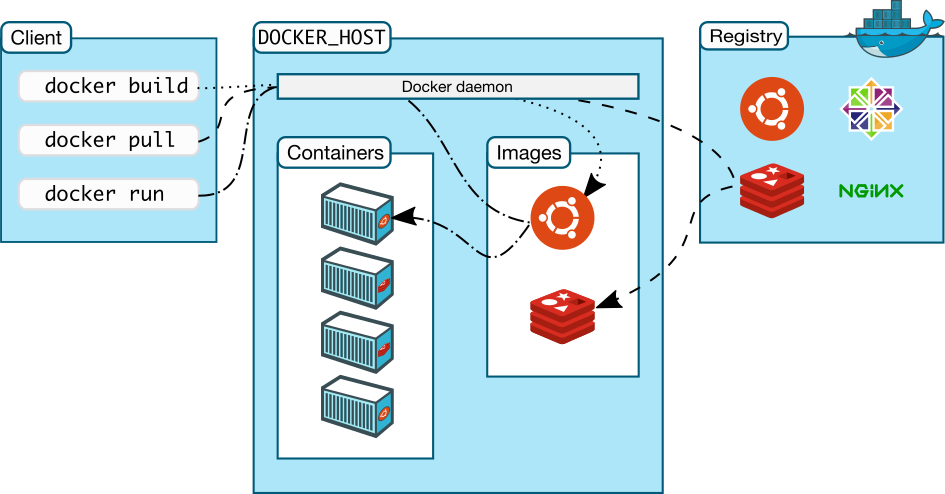
\includegraphics[width=0.8\textwidth]{../imgs/EdA/docker-arch.png}
	\caption{Arquitectura del sistema de contenedores Docker}
	\label{fig:docker-arch}
	\end{figure}
	
	\begin{figure}[h]
	\centering
	
\includegraphics[width=0.2\textwidth]{../imgs/EdA/docker.png}
	\caption{Logo de Docker}
	\label{fig:docker-logo}
	\end{figure}

	En el ciclo de vida de un contenedor Docker podemos distinguir 5 estados principales:

	\begin{itemize}
		\item \textbf{Created:} hace referencia a un contenedor que ha sido creado pero no arrancado.
		\item \textbf{Running/Started:} contenedor corriendo con todos sus procesos.
		\item \textbf{Paused:} contenedor cuyos procesos se han pausado usando la señal SIGSTOP de cgroups.
		\item \textbf{Stopped/Exited:} contenedor cuyos procesos se han parado. La diferencia con \textit{paused} es que se libera la memoria que estaban usando los procesos que han sido detenidos, usando la señal SIGKILL de cgroups. El sistema de ficheros se mantiene tal y como estaba en el momento que se detuvo el contenedor.
		\item \textbf{Deleted/Dead:} contenedor eliminado. Es posible recuperarlo durante un periodo de tiempo determinado.
	\end{itemize}

	\begin{figure}[h]
	\centering
	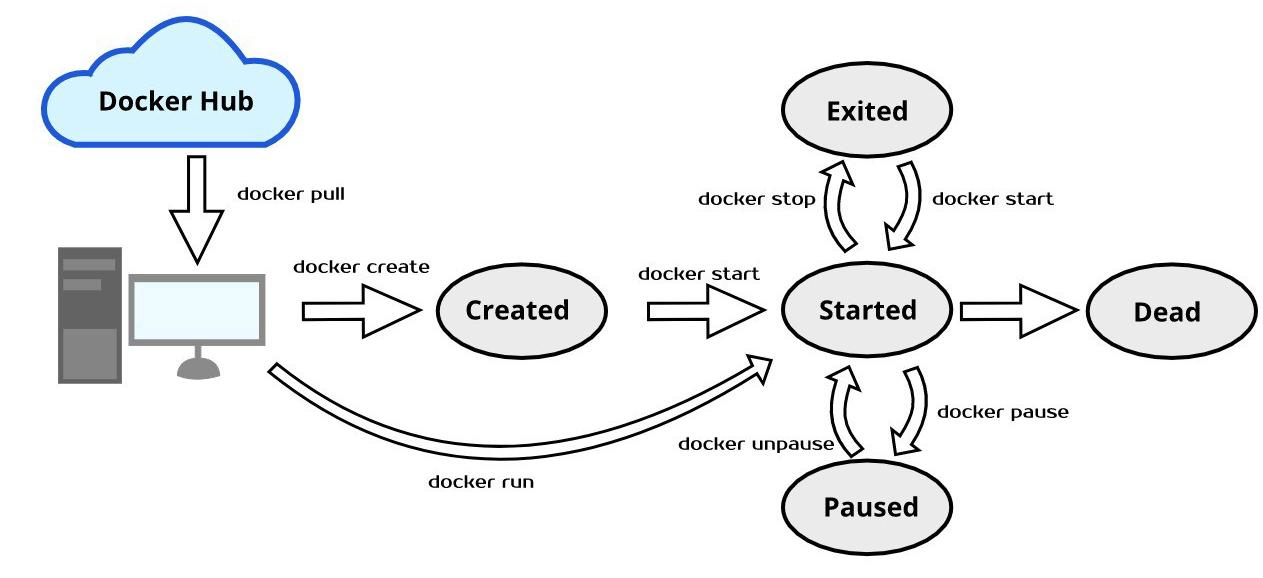
\includegraphics[width=0.8\textwidth]{../imgs/EdA/docker-life.jpeg}
	\caption{Ciclo de vida de los contenedores Docker}
	\label{fig:docker-life}
	\end{figure}

	Como se puede apreciar en la figura, Docker permite gestionar el estado de los contenedores de forma sencilla mediante la CLI, algunas de sus órdenes más destacadas son:

\begin{lstlisting}[language=bash]
  $ docker pull #permite descargar una imagen de un repositorio
  $ docker create #crea un nuevo contenedor, pero no lo arranca 
  $ docker start #arranca contenedores parados
  $ docker run #es equivalente a create + start
  $ docker stop #detiene los procesos corriendo en un contenedor  
  $ docker pause #pausa los procesos corriendo en un contenedor
  $ docker unpause #reanuda la ejecucion de los procesos pausados
  $ docker rm #elimina los procesos y el contenedor donde corrian
\end{lstlisting}

\subsubsection{Diferencias entre LXC y Docker}
	Con todo esto, podemos sacar varias conclusiones importantes acerca de estos dos tipos de contenerización, que condicionarán la elección de uno u otro en función de su uso. La principal sería que mientras que con LXC se virtualiza un sistema operativo completo, con Docker se virtualizan aplicaciones. Además, los contenedores LXC sólo permiten virtualizar entornos Linux y no se pueden portar entre máquinas, mientras que Docker permite portar entre máquinas e incluso plataformas. Esto último es algo relevante puesto que si en algún momento fuese necesario migrar a otro entorno, gracias a la portabilidad de Docker nos ahorraremos el tener que instalar en este nuevo entorno todas aquellas aplicaciones que normalmente usemos. 

	Finalmente, también cabe recalcar que LXC proporciona un menor aislamiento del sistema operativo respecto a Docker. Al virtualizar sistemas operativos completos y aislados dentro del mismo host, debe haber usuario root y llamadas al propio sistema operativo (si no fuese así, estaríamos ante un sistema «recortado» porque no se podrían hacer determinadas cosas). Docker sirve para virtualizar aplicaciones dentro de un mismo host, por lo que el nivel de acceso root sí puede estar más limitado y controlado, lo que lo hace más seguro.

	\vspace{0.2cm}
	\begin{figure}[h]
	\centering
	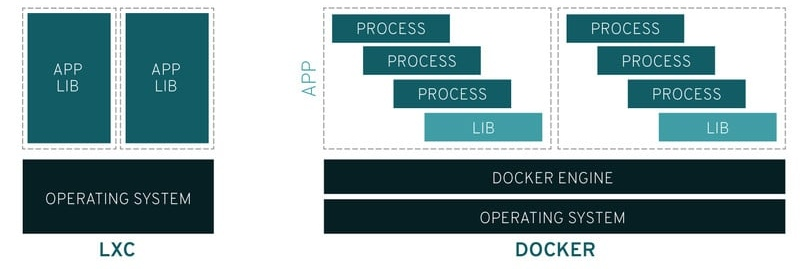
\includegraphics[width=0.8\textwidth]{../imgs/EdA/LXCvsDocker.jpg}
	\caption{Docker vs LXC: Estructura}
	\label{figure:LXCvsDocker}
	\end{figure}
	\clearpage

\section{Tecnologías de aprovisionamiento} \label{sec:aprov}
	Antes de entrar en materia, se va a presentar la infraestructura como código, un concepto fundamental para el desarrollo de este trabajo. 

	La infraestructura como código (IaC) permite gestionar y preparar la infraestructura de un entorno con código, en lugar de hacerlo mediante procesos manuales. Con este tipo de infraestructura, se crean archivos de configuración que contienen las especificaciones que esta necesita, lo cual facilita la edición y la distribución de las configuraciones. Asimismo, garantiza que siempre se despliegue el mismo entorno.~\cite{aprov1}

	La IaC se puede abordar mediante dos enfoques: uno declarativo o uno imperativo:

	\begin{itemize}
		\item \textbf{Enfoque declarativo:} define el estado deseado del sistema, incluidas las propiedades que debe tener y los recursos necesarios, y la herramienta de IaC se encarga de configurarlo.
		\item \textbf{Enfoque imperativo:} define los comandos específicos para lograr la configuración deseada, los cuales se deben ejecutar en el orden correcto.
	\end{itemize}

	Las tecnologías de virtualización presentadas en el apartado anterior recibirán órdenes del orquestador de escenario (herramienta IaC que veremos más adelante) para desplegar las máquinas necesarias para formar un escenario de red determinado. 

	Por tanto, podemos decir que el aprovisionamiento consiste en la instalación y la configuración del software (incluido el sistema operativo y las aplicaciones) necesario para que dichas máquinas puedan desempeñar su función en el escenario de red. No es lo mismo que la configuración, aunque ambos son pasos en el proceso de implementación.

	Dentro del aprovisionamiento podríamos diferenciar dos tipos, que están muy ligados a los distintos enfoques de la IaC. El primero sería un aprovisionamiento “en frío” o estático, en el que se abastece la máquina antes de arrancarla y levantar el escenario. Por otro lado tendríamos el aprovisionamiento “en caliente” o dinámico, cuya idea principal reside en  lanzar órdenes, comandos o depositar archivos en una máquina ya levantada y arrancada.

\subsection{Aprovisionamiento estático} \label{sec:est}
	Este tipo de aprovisionamiento tiene un enfoque imperativo, y, como ya se ha mencionado, se basa en crear de manera offline la máquina con todo lo necesario ya instalado, de forma que cuando se despliegue sólo requiera algunas pequeñas modificaciones adicionales, como podrían ser configuraciones de red. A continuación se va a detallar el uso de Docker y Vagrant para el aprovisionamiento, pero hay otras alternativas a tener en cuenta como las ISO/OVA  de VirtualBox.

\subsubsection{Docker}
	Habíamos visto, en el apartado de virtualización basada en contenedores, que una imagen Docker es una instantánea de la aplicación o servicio que corre en un contenedor y de su configuración y las dependencias. En otras palabras, una imagen es un archivo, compuesto por múltiples capas, que constituye una representación estática del estado de un contenedor.

	Estas imágenes son las plantillas base desde la que partimos ya sea para crear una nueva imagen o crear nuevos contenedores para ejecutar las aplicaciones. Las imágenes pueden ser locales si se almacenan en el host, o remotas si se suben a repositorios públicos como DockerHub, donde cualquier usuario que lo desee puede hacer uso de ellas. En los repositorios se pueden encontrar tanto imágenes oficiales desde las que partir como imágenes de terceros ya modificadas.

	Para crear nuestras propias imágenes, donde dotemos a nuestros contenedores del software así como de su configuración necesaria, Docker nos proporciona los Dockerfile. Un Dockerfile es un archivo de texto plano que contiene una serie de instrucciones necesarias para armar una imagen. A partir de esa imagen podemos crear varias instancias o contenedores, que integran todo lo necesario para ejecutar una aplicación.

	\begin{figure}[h]
	\centering
	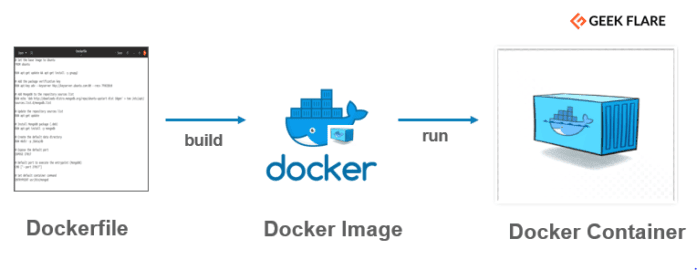
\includegraphics[width=0.8\textwidth]{../imgs/EdA/dockerfile.png}
	\caption{Creación de un contenedor Docker a partir de un Dockerfile}
	\label{fig:dockerfile}
	\end{figure}

	Una imagen de Docker consiste en una serie de capas de “solo-lectura”, cada una de las cuales se representa con una instrucción del Dockerfile. Las capas se amontonan unas sobre otras y cada una añade algo sobre la anterior. Cuando creamos un contenedor, que no es más que una instancia en ejecución de una imagen, estamos añadiendo una capa escribible encima de todas las demás capas de solo-lectura. Así, la estructura de una imagen Docker se podría representar como sigue: \\ 

	\begin{figure}[h]
	\centering
	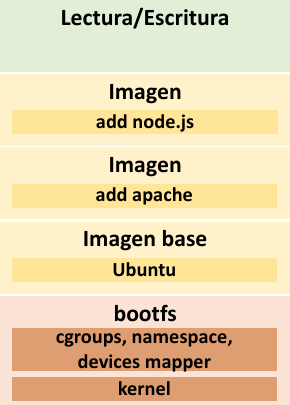
\includegraphics[width=0.3 \textwidth]{../imgs/EdA/dockerfile2.png}
	\caption{Representación de las capas de un Dockerfile}
	\label{fig:dockerfile-layers}
	\end{figure}

	La imagen tendrá una base mínima, que han de tener todas las imágenes para el correcto funcionamiento del contenedor. Esta base incluye el kernel y algunas de sus características necesarias de las que ya hemos hablado como cgroups y namespaces. Encima de la base se representan las capas de sólo lectura, que serían las instrucciones del Dockerfile. En este ejemplo se parte de una imagen Ubuntu a la que se le instala nodejs y apache. Finalmente al crear el contenedor con la instrucción docker run se añade la última capa, correspondiente a los sistemas de ficheros de lectura/escritura, sobre el resto de capas, de forma que podemos interactuar con el contenedor.

	% La sintaxis de un Dockerfile es sencilla y flexible. Cada instrucción va en una fila, siguiendo el formato \texttt{<INSTRUCCIONES> <ARGUMENTOS>}, y se ejecuta de manera independiente a las demás. En el Dockerfile del ejemplo anterior se han usado las instrucciones \texttt{FROM} para indicar que se parte de una imagen base Ubuntu, y \texttt{RUN} para ejecutar comandos en la imagen (correspondientes a la instalación de los paquetes de apache y node). Pero hay multitud de instrucciones más, como por ejemplo \texttt{ENV} para establecer variables de entorno persistentes en el contenedor o \texttt{COPY} para copiar archivos o directorios de la máquina host al contenedor. Cuando construyamos nuestras propias imágenes, se profundizará más en estas instrucciones y su funcionamiento.

\subsubsection{Vagrant}
	Vagrant~\cite{vagrant} es una herramienta de línea de comandos que permite crear y configurar máquinas virtuales a partir de ficheros de configuración llamados Vagrantfile.

	\begin{figure}[h]
	\centering
	
\includegraphics[width=0.2 \textwidth]{../imgs/EdA/vagrant.png}
	\caption{Logo de Vagrant}
	\label{fig:vagrant}
	\end{figure}

	Al poseer estos ficheros de configuración, que nos permiten definir los servicios a instalar así como también sus configuraciones, se centraliza toda la configuración de la VM que creamos, de forma que es  posible  utilizar el mismo Vagrantfile para crear una VM exactamente igual cuantas veces se quiera. Esto es algo muy ventajoso ya que nos permite ahorrar la carga de trabajo que supone el desplegar el mismo entorno una y otra vez, con la seguridad de que nuestro entorno siempre tendrá la misma configuración.

	Cabe destacar que vagrant no tiene la capacidad para correr una máquina virtual sino que simplemente se encarga de definir las características con las que debe crearse esa VM y los complementos a instalar. Para poder trabajar con las máquinas virtuales es necesario la instalación de VirtualBox, Docker, Hyper-v, o la tecnología de virtualización que se desee (y sea compatible\footnote{Ver en la documentación oficial~\cite{vagrant}}).

        % WARNING
% 	Desde Vagrant se pueden configurar algunos aspectos de la máquina virtual relacionados con la red, los puertos y hasta la IP, aunque se requiere para ello la instalación de una serie de servicios en el sistema operativo. Si no se instalaran estos servicios, no se podría hacer desde Vagrant y se debería usar alguna otra herramienta, como por ejemplo Ansible, la cual veremos más adelante.

% 	Un ejemplo sencillo de Vagrantfile sería el siguiente:~\cite{vagrant2}
%
% \begin{lstlisting}[language=Bash, caption=Ejemplo de Vagrantfile]
% 	Vagrant.configure("2") do |config|
% 	    config.vm.box = "genebean/centos6-64bit"
% 	    # network
% 	    config.vm.network "private_network", ip: "192.168.56.100"
% 	    # hardware
% 	    config.vm.provider "virtualbox" do |vb|
% 	        vb.memory = "1024"
% 	        vb.cpus = 1
% 	    end
%
% 	    config.vm.provision "shell", inline: <<-SHELL
% 	        yum update
% 	        yum install -y nginx
% 	        yum install -y epel-release
% 	        rpm -Uvh https://mirror.webtatic.com/yum/el6/latest.rpm
% 	        yum install -y php56w-fpm php56w-opcache
% 	        yum replace php-common --replace-with=php56w-common
% 	        yum -y install --enablerepo=remi,remi-test mysql mysql-server
% 	   SHELL
% 	end 
% \end{lstlisting}
%
% 	La instrucción \texttt{vagrant up} usaría este fichero para crear una VM en VirtualBox con 1 CPU y una memoria de 1024 MB partiendo de una imagen Centos 6 de 64bit, en la que se realiza la instalación de Nginx, PHP 5.6 y MariaDB utilizando un shell script. El aprovisionamiento sólo se ejecuta al crear la máquina, todas las demás veces que se inicie la máquina virtual no se ejecutará este script, a no ser que se indique expresamente mediante el comando \texttt{vagrant provision}. Una vez creada, bastaría con la orden \texttt{vagrant ssh} para acceder a ella o bien podríamos detenerla o eliminarla con \texttt{vagrant halt} y \texttt{vagrant destroy}, respectivamente.
	
	Vagrant permite realizar algunas configuraciones de red, pero no está pensado para trabajar con grandes cantidades de máquinas virtuales, para infraestructuras más complejas existen otras herramientas como Terraform que pertenece a la misma empresa HashiCorp, y que vamos a presentar posteriormente como una de las tecnologías de orquestación de escenarios.

        En resumen, Vagrant es muy fácil de instalar y utilizar, permitiéndonos configurar entornos locales solo con un par de comandos. Además, nos proporciona la seguridad de que todos los entornos que creemos con el mismo Vagrantfile serán iguales. Como desventaja, es importante que todos los comandos a ejecutar no necesiten la interacción del usuario, ya que si no, va a fallar.

	\clearpage

\subsection{Aprovisionamiento dinámico} \label{sec:din}
	El enfoque imperativo de las herramientas presentadas en el apartado anterior, así como de los tradicionales scripts en bash o python empleados para automatizar configuraciones, donde se detallan todas las instrucciones necesarias para llegar a la configuración deseada, puede desembocar en errores de ejecución. 

	Imaginemos un script en el que uno de los pasos para lograr la configuración deseada es crear un directorio. La primera vez que se ejecute, este script funcionará correctamente, pero, si lo volvemos a ejecutar, lo más seguro es que aparezca un error debido a que el directorio ya se creó al ejecutar el script por primera vez, y estaríamos intentando crear un directorio ya existente. 

	Para evitar este problema y derivados provocados por errores humanos, es muy común el empleo de un aprovisionamiento dinámico, mediante herramientas de gestión de configuración. La principal característica que presentan estas herramientas es lo que se conoce como idempotencia, que se define como la propiedad para realizar una acción determinada varias veces y aún así conseguir el mismo resultado que se obtendría si se realizase una sola vez.
	
	\begin{figure}[h]
	\centering
	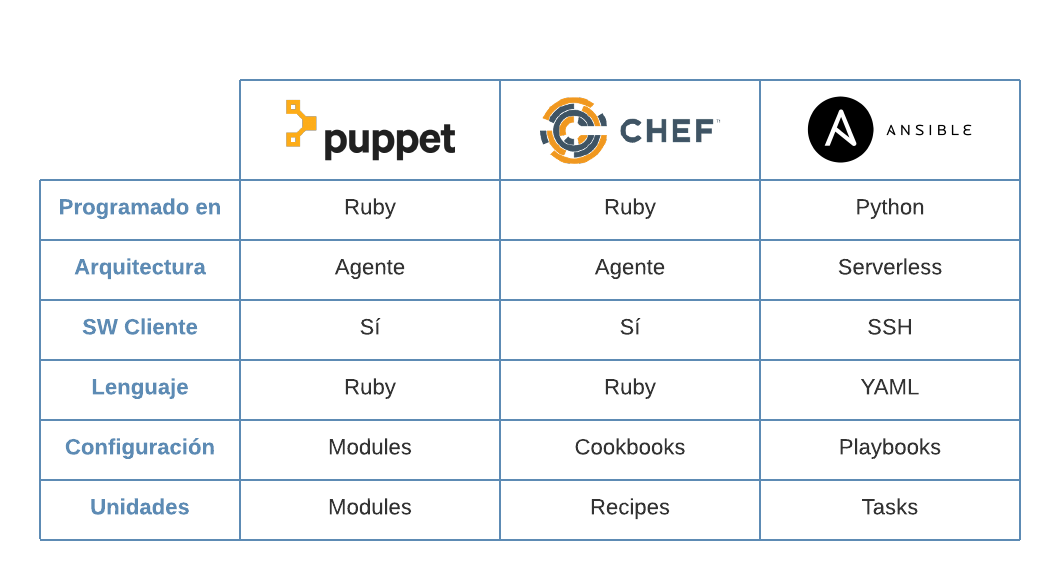
\includegraphics[width=0.8\textwidth]{../imgs/EdA/aprovisionamiento.png}
	\caption{Comparativa de herramientas de gestión de la configuración}
	\label{fig:aproVS}
	\end{figure}

	Esto es debido a que las herramientas de gestión de la configuración usan un lenguaje declarativo, en el que simplemente hay que especificar el estado final deseado, y la propia herramienta llevará a cabo las acciones necesarias para llegar a él, que variarán en función del estado en el que se encuentre la máquina. De esta forma se agilizan los cambios y las implementaciones, se elimina la posibilidad de que se cometan errores humanos, y la gestión del sistema se torna predecible y ajustable.~\cite{aprov2}

	Además, estas herramientas posibilitan también tener la configuración de una infraestructura TI en forma de código, lo que da lugar a que una infraestructura sea:

	\begin{itemize}
		\item \textbf{Escalable.} La automatización del proceso de configuración ofrece la ventaja de poder aplicarlo tanto a infraestructuras pequeñas como de gran tamaño.
		\item \textbf{Replicable.} El código puede ser replicado y a partir de él generar la infraestructura, de manera que se adapten según las necesidades y entornos disponibles.
	\end{itemize}

	Actualmente existen una gran variedad de herramientas de este tipo (ver figura \ref{fig:aproVS}) con diferentes características.

\subsubsection{Chef}
	El software Chef~\cite{chef1} es una herramienta de gestión de la configuración de código abierto que permite crear partes de una infraestructura como un servicio. Para ello hace uso de tres elementos principales:~\cite{chef2}
	\begin{itemize}
		\item \textbf{Recipes.} Una receta es un fichero escrito en Ruby que contiene el código que va a realizar operaciones sobre las máquinas, en este caso sería la gestión de software y configuración, aunque también podría realizarse el despliegue. Una receta puede depender o estar contenida en otra.
		\item \textbf{Cookbooks.} Un libro de cocina es la unidad fundamental de configuración y distribución de políticas. Define un escenario y contiene todo lo necesario para que se de ese escenario: recetas que especifican los recursos a utilizar, atributos para sobrescribir la configuración predeterminada de una máquina, ficheros estáticos para administrar archivos de configuración…
		\item \textbf{Knife.} Desde las estaciones de trabajo o workstations se gestionan las configuraciones antes de enviarlas al Chef Server. Para ello se emplea una herramienta de línea de comandos llamada Knife que permite interactuar mediante SSH con el servidor Chef. Con Knife se puede subir, descargar o eliminar cookbooks de Chef Server, instalar Chef Client en dispositivos (crear nodos), consultar datos acerca de nodos y cookbooks etc.
	\end{itemize}

	Chef es de tipo cliente-servidor, por lo que es necesaria la instalación y configuración del software Chef Client en los nodos o dispositivos (ya sean físicos, virtuales, o en la nube) que se quieran aprovisionar. Una vez instalado, todos los nodos gestionados se comunican con el servidor principal a través del uso de certificados. El elemento principal y núcleo es el llamado Chef Server, desde el cual es posible centralizar el proceso de lanzamiento y configuración de las máquinas haciendo uso de los cookbooks y recetas almacenadas en él.

	\begin{figure}[h]
	\centering
	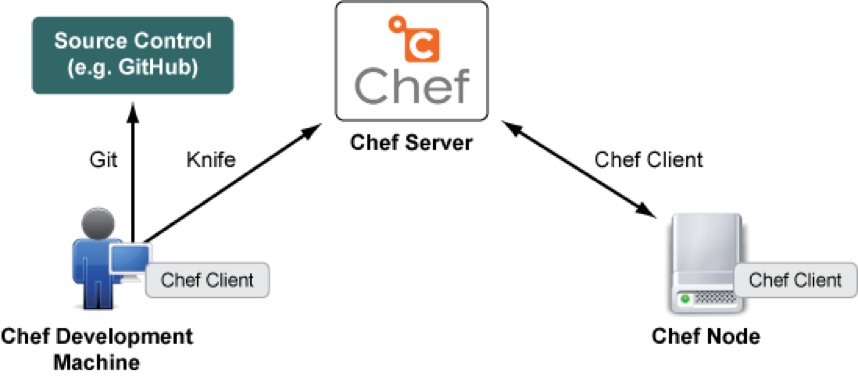
\includegraphics[width=0.8\textwidth]{../imgs/EdA/arquitectura-chef.png}
	\caption{Arquitectura de funcionamiento de Chef}
	\label{fig:chef-arch}
	\end{figure}
	\clearpage

\subsubsection{Ansible}
	Ansible~\cite{ans1}, al igual que Chef, es un motor open source que automatiza los procesos para preparar la infraestructura, gestionar la configuración, implementar las aplicaciones y organizar los sistemas, entre otros procedimientos de TI.

	Ansible está escrito en Python, y presenta algunas ventajas respecto a Chef. En primer lugar es serverless, lo que significa que no hay que instalar agentes ya que la configuración se lleva a cabo por SSH. Además, la configuración se realiza en YAML, un lenguaje más sencillo de aprender y usar que Ruby. Todo esto hace que la curva de aprendizaje en Ansible sea considerablemente menor que la de Chef y Puppet.

	En Ansible también podemos destacar tres elementos principales:

	\begin{itemize}
		\item \textbf{Inventario.} Es un fichero YAML que contiene el grupo de máquinas sobre las que se va a realizar una acción determinada.
		\item \textbf{Task.} Una tarea o task es la acción específica a realizar sobre las máquinas (el estado en el que queremos que quede el sistema). Sólo es necesario declarar el estado final, ya que como se había comentado estas herramientas tienen un enfoque declarativo. Cada tarea no es más que una llamada a un módulo de Ansible.
		\item \textbf{Playbook.} un playbook es un fichero YAML que contiene una lista de plays o actos, siendo un play una lista de tareas o tasks que se aplican sobre un determinado conjunto de hosts (inventario).
	\end{itemize}
	
	\vspace{0.2cm}
	\begin{figure}[h]
	\centering
	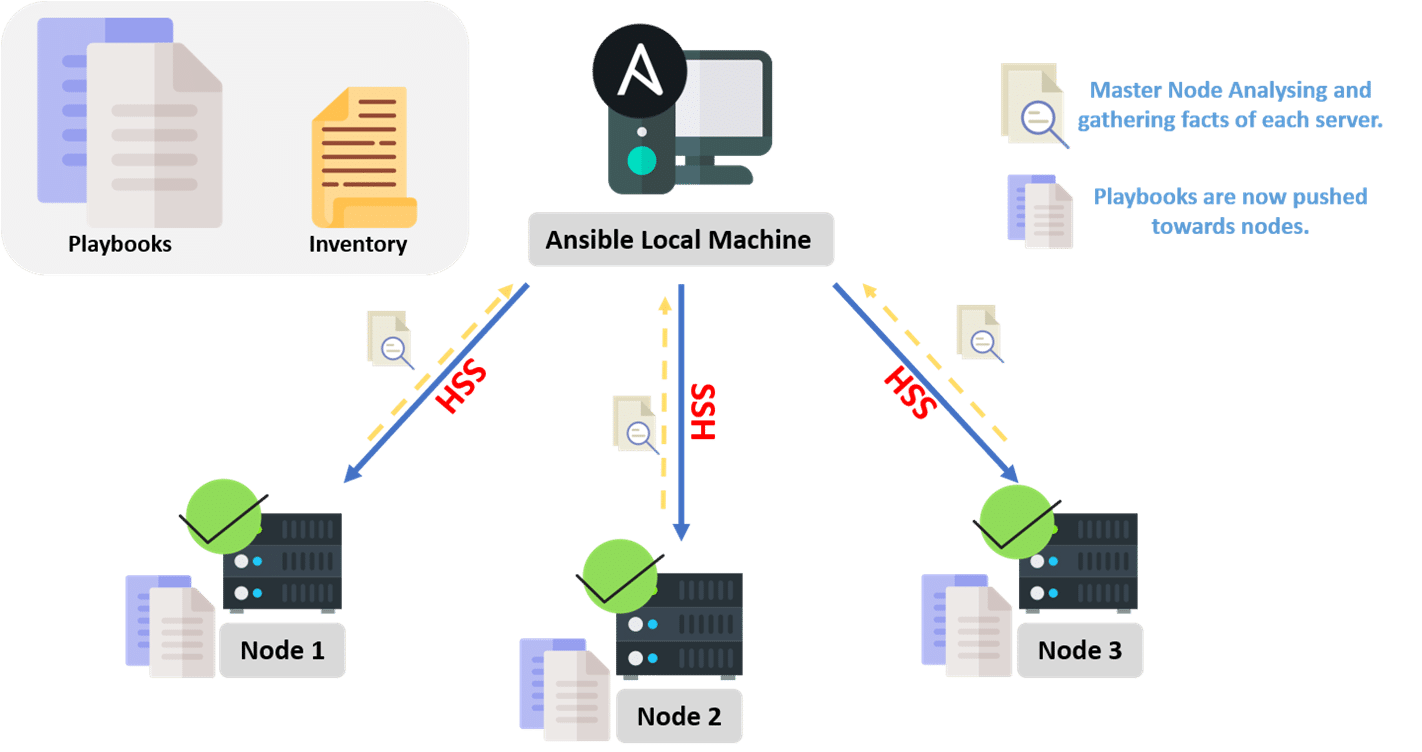
\includegraphics[width=0.8\textwidth]{../imgs/EdA/arquitectura-ansible.png}
	\caption{Arquitectura de funcionamiento de Ansible}
	\label{fig:ansible-arch}
	\end{figure}

	La ventaja principal de Ansible frente al resto de herramientas de configuración es su facilidad de uso. Para su funcionamiento es necesario que el cliente cuente con SSH y Python, que normalmente suelen estar instaladas por defecto en los sistemas Linux. 
        
        % WARNING
%       Vamos a ver a continuación un ejemplo en el que se actualiza un servidor web con Ansible. En primer lugar habría que crear un fichero (en este ejemplo se llama \textit{inventory.ini}) con el host a actualizar, que previamente tendremos que haber definido en el fichero \texttt{/etc/hosts} para que la resolución de dominio sea correcta (en su defecto, tendríamos que especificar la dirección IP en el inventario). Su contenido podría ser el siguiente:
% 	
% \clearpage
% \begin{lstlisting}[language=Bash, caption=Contenido del fichero inventory.ini]
% 	[webserver]
% 	ansible_host=192.168.1.2 ansible_user=ubuntu ansible_password=daerv
% \end{lstlisting}	
% 	
% 	Lo conveniente, por temas de seguridad, habría sido el uso de keypairs en vez de poner la contraseña, pero para facilitar el entendimiento del ejemplo se muestra así. Ahora habría que definir un playbook (\textit{ansible.yml}) con las tasks a realizar en ese host:
%
% \vspace{0.2cm}
% \begin{lstlisting}[language=Bash, caption=Contenido del fichero ansible.yml]
% 	---
% 	- hosts: webserver
% 	  tasks:
% 	  - name: Actualizar Apache 
% 	    apt: name=apache2 state=latest
% 	  - name: Apache corriendo  
% 	    service: name=apache2 state=restarted
% \end{lstlisting}
%
% 	La comunicación entre la máquina de control y las administradas es vía SSH. Por tanto, la máquina de control deberá tener la clave privada y las máquinas administradas la clave pública. Si esto se cumple, correríamos el playbook mediante la siguiente orden:
%
% \vspace{0.2cm}
% \begin{lstlisting}[language=Bash, caption=Orden de ejecución del playbook de Ansible]
%         		$ ansible-playbook ansible.yml -i inventory.ini 
% \end{lstlisting}
\clearpage

\section{Tecnologías de orquestación} \label{sec:orq}
	En el pasado, la preparación de la infraestructura de TI se llevaba a cabo de forma manual e incluía la instalación de servidores físicos y la configuración del hardware según los ajustes deseados. Si se necesitaba más capacidad, se tenía que solicitar más hardware, esperar a que llegara y luego instalarlo y prepararlo.~\cite{orq1} 

	En la actualidad, la infraestructura suele definirse en el software. La virtualización y los contenedores agilizaron los procesos de preparación y eliminaron la necesidad de preparar y gestionar sistemas de hardware con frecuencia. Al igual que el aprovisionamiento de las máquinas, la preparación del escenario también puede automatizarse.

	Las herramientas de orquestación de escenario son una tecnología IaC mediante la cual es posible definir vía fichero qué elementos a nivel de red/arquitectura se van a desplegar: máquinas, VLANs, recursos dedicados (como cantidad de CPU y memoria), etc. 

	Al presentar las tecnologías de virtualización y aprovisionamiento hablamos de despliegue, que es el hecho de levantar y configurar (por ejemplo, a nivel interconexión de red) las máquinas que van a formar ese escenario virtualizado. Por tanto, si se combina la orquestación de escenario junto con el despliegue, ambas tecnologías IaC, podremos realizar el despliegue automatizado de escenarios de red virtualizados.

\subsection{Docker Compose}
	Docker Compose~\cite{orq2} es una herramienta para definir y ejecutar múltiples contenedores Docker de forma simultánea en un mismo host. Utiliza un archivo YAML (normalmente de nombre \texttt{docker-compose.yml}) para configurar los servicios de la aplicación. Luego, con un solo comando, crea e inicia todos los servicios desde su configuración. Si bien en algunos casos se puede decir que es un orquestador, no es del todo comparable a los orquestadores que veremos a continuación (como ECS, Kubernetes, etc) ya que pese a que puede ejecutar varios servicios distintos, no puede manejar autoscaling, downtime etc.

	\begin{figure}[h]
	\centering
	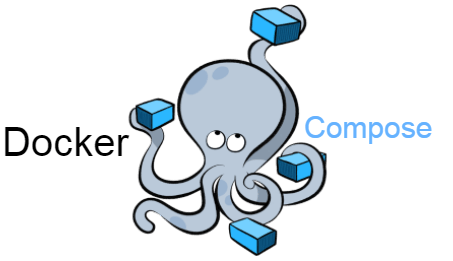
\includegraphics[width=0.5\textwidth]{../imgs/EdA/compose.png}
	\caption{Logo de Docker Compose}
	\label{fig:compose}
	\end{figure}

	El fichero Dockerfile del que hablamos en el apartado \ref{sec:aprov} define como crear la imagen de una aplicación o contenedor, mientras que el fichero \textit{docker-compose.yml} nos permite vincular y configurar estos contenedores en conjunto para construir varios servicios. La forma en que ejecutamos nuestro docker compose es con la instrucción \texttt{docker-compose up}, el cual entrega instrucciones para ejecutar el contenedor según el \textit{docker-compose.yml}.

\subsection{Kubernetes}
	Docker Compose nos permite desplegar múltiples contenedores en un mismo host. Es posible que, por motivos de disponibilidad entre otros, quisiéramos tener nuestros contenedores ejecutándose en diferentes hosts. Esto, entre otras cosas (como que los host que alojan estos contenedores estén en la nube), es algo que nos permite Kubernetes.

	Kubernetes~\cite{orq3} es un orquestador open source para aplicaciones que se ejecutan en contenedores de software. La ventaja principal de usar Kubernetes es que facilita enormemente la gestión de los contenedores al encargarse del trabajo duro en el escalamiento, recuperación automática, balanceo de cargas, despliegues y mucho más. 

	% WARNING
	% La siguiente figura muestra una recapitulación de todos los tipos de despliegue que se han explicado hasta ahora. Esta contextualización permite un mejor entendimiento del concepto de Kubernetes y de las tecnologías de orquestación en general.

	% \vspace{0.2cm}
	% \begin{figure}[h]
	% \centering
	% 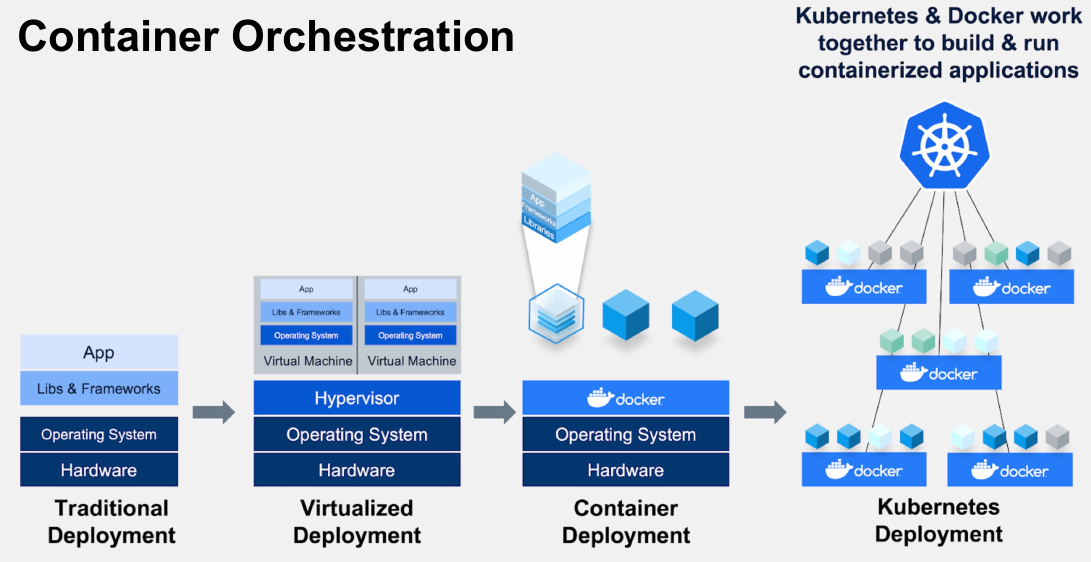
\includegraphics[width=0.8\textwidth]{../imgs/EdA/k8s-1.png}
	% \caption{Orquestación de contenedores con Kubernetes}
	% \label{fig:k8s}
	% \end{figure}

	Los elementos principales de Kubernetes son los siguientes:

	\begin{itemize}
		\item \textbf{Plano de control.} Conjunto de procesos que controlan los nodos de Kubernetes. Es donde se originan todas las asignaciones de tareas.
		\item \textbf{Nodo.} Máquina física o virtual que ejecuta las tareas asignadas por el plano de control.
		\item \textbf{Clúster.} Conjunto de nodos. Es lo que sería una implementación de Kubernetes en funcionamiento.
		\item \textbf{Pod.} Conjunto de contenedores que se ejecutan en el mismo nodo, compartiendo volumen y network namespace (IP, hostname, etc).
		\item \textbf{Controlador de replicación.} Controla la cantidad de copias idénticas de un pod que deben ejecutarse en algún lugar del clúster.
		\item \textbf{Servicio.} Separa las definiciones de las tareas de los pods. Los proxies de servicios de Kubernetes envían las solicitudes de servicio al pod correspondiente de forma automática, sin importar a dónde se traslade en el clúster ni si se lo reemplaza.
		\item \textbf{Kubelet.} Servicio que se ejecuta en los nodos y se encarga de leer los manifiestos del contenedor y de garantizar el inicio y el funcionamiento de los contenedores definidos.
	\end{itemize}

	\begin{figure}[h]
	\centering
	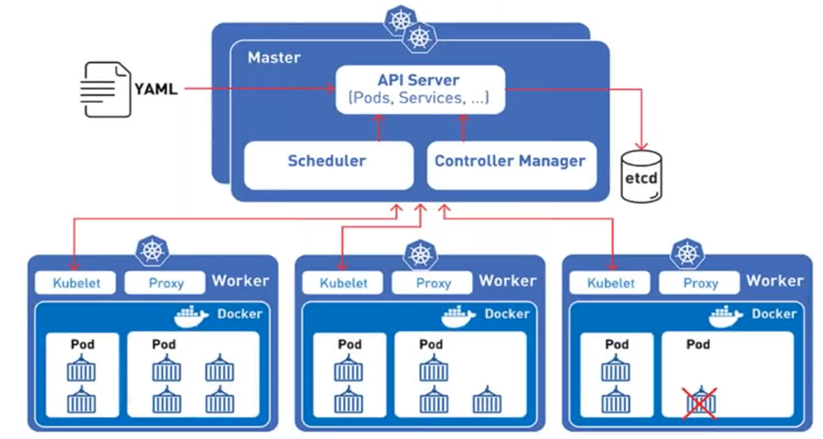
\includegraphics[width=0.8\textwidth]{../imgs/EdA/k8s-arch.png}
	\caption{Arquitectura de Kubernetes}
	\label{fig:k8s}
	\end{figure}

\subsection{Terraform}
	Terraform~\cite{orq4} es una herramienta open-source de codificación declarativa desarrollada por HashiCorp que permite describir la infraestructura de estado final deseada para ejecutar una aplicación en local o en cloud. Esto se hace mediante ficheros de configuración en formato JSON o en la sintaxis de alto nivel HCL (HashiCorp Configuration Language) propuesta por Terraform. 

	Una vez especificado el estado deseado, elabora un plan para alcanzar ese estado final y lo ejecuta para suministrar la infraestructura.

	La infraestructura que Terraform puede administrar incluye componentes de bajo nivel, como instancias informáticas, almacenamiento y redes, así como componentes de alto nivel como entradas de DNS, características de SaaS, etc.

	Lo más común es usar un fichero para definir la arquitectura, una serie de variables para poder parametrizar el despliegue y algunas variables de salida para obtener los datos más importantes de la infraestructura una vez desplegada (por ejemplo la IP de un ELB de AWS o el endpoint de RDS).

	Existen cuatro elementos principales en Terraform:
	
	\begin{itemize}
		\item \textbf{Providers:} definen los elementos data y resources para plataformas y herramientas específicas. Son plugins que implementan tipos de recursos y contienen todo el código necesario para autenticar y conectarse a un servicio, normalmente desde un proveedor de cloud público, en nombre del usuario. Es posible encontrar proveedores para las plataformas y servicios de cloud que se vayan a utilizar, añadirlos a la configuración y, a continuación, utilizar sus recursos para suministrar la infraestructura. Los proveedores están disponibles para casi todos los principales proveedores de cloud, oferta de SaaS, y más, desarrollados y/o soportados por la comunidad de Terraform u organizaciones individuales.
		\item \textbf{Resources:} definen elementos de la infraestructura que pueden ser aprovisionados, junto con sus propiedades. Una vez desplegados, proporcionan salidas que pueden utilizarse como entrada de otros elementos o como salida final de la ejecución, para mostrar al usuario.
		\item \textbf{Data:} recuperan información acerca del estado actual de un recurso u otro elemento y proporcionan salidas.
		\item \textbf{Modules:} son abstracciones para agrupar conjuntos de data y resources. Se pueden configurar entradas y salidas. Los módulos de Terraform son pequeñas configuraciones de Terraform reutilizables para varios recursos de infraestructura que se utilizan conjuntamente. Son útiles porque permiten automatizar recursos complejos con construcciones configurables y reutilizables. Escribir incluso un archivo de formato Terraform muy simple genera un módulo. Un módulo puede llamar a otros módulos, denominados módulos hijo, que permiten que la configuración de ensamblaje sea más rápida y concisa. Los módulos también se pueden llamar varias veces, ya sea dentro de la misma configuración o en configuraciones separadas.
	\end{itemize}
	\clearpage

	\begin{figure}[h]
	\centering
	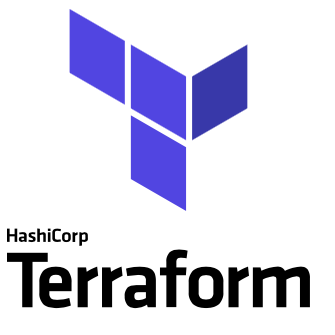
\includegraphics[width=0.3\textwidth]{../imgs/EdA/terraform.png}
	\caption{Logo de Terraform}
	\label{fig:terraform}
	\end{figure}

	Hay algunas razones clave por las cuales los desarrolladores eligen utilizar Terraform sobre otras herramientas de Infraestructura como código:~\cite{orq5}

	\begin{itemize}
		\item \textbf{Open Source.} Terraform está respaldada por grandes comunidades de colaboradores que crean plugins para la plataforma. Independientemente del proveedor de cloud que se utilice, es fácil encontrar plugins, extensiones y soporte profesional. Esto también significa que Terraform evoluciona rápidamente y constantemente se añaden nuevas ventajas y mejoras.
		\item \textbf{Plataforma agnóstica.} Esto significa que puede ser utilizada con cualquier proveedor de servicios de cloud. La mayoría de las demás herramientas de IaC están diseñadas para funcionar con un único proveedor de cloud, lo que podría ser visto como una desventaja ya que si quisiéramos migrar nuestra infraestructura a otro proveedor habría que reescribir gran parte del código.
		\item \textbf{Infraestructura inmutable.} La mayoría de las herramientas de Infraestructura como código crean una infraestructura mutable, lo que significa que la infraestructura puede cambiar para acomodar cambios como una actualización de middleware o un nuevo servidor de almacenamiento. El peligro con la infraestructura mutable es la desviación de configuración, a medida que los cambios se acumulan, el suministro real de diferentes servidores u otros elementos de infraestructura 'se desvía' más allá de la configuración original, haciendo que los errores o problemas de rendimiento sean difíciles de diagnosticar y corregir. Terraform suministra una infraestructura inmutable, lo que significa que con cada cambio en el entorno, la configuración actual se sustituye por una nueva que aplica el cambio y se vuelve a suministrar la infraestructura. Incluso mejor, se pueden conservar las configuraciones anteriores como versiones para habilitar las reversiones en caso necesario o si así se desea.
		\item \textbf{Lenguaje sencillo.} El lenguaje de configuración de alto nivel que propone HashiCorp, HCL, es muy fácil de entender ya que es muy cercano al lenguaje natural. De esta forma, la sintaxis no es un aspecto que entorpezca el aprendizaje.
	\end{itemize}
	\clearpage

% WARNING
% \subsubsection{Tecnologías de orquestación de proveedores cloud}
% 	Las herramientas que se han presentado son muy utilizadas por las funciones que ofrecen y la cantidad de trabajo que facilitan. Es por esto que los principales proveedores cloud cuentan con servicios (ver figura \ref{fig:cloud}) que bien permiten la integración con estas herramientas o que proporcionan funcionalidades muy similares. Se han clasificado estos servicios en dos tipos:
%
% 	\begin{itemize}
% 		\item \textbf{Servicio declarativo:} permite modelar y configurar los recursos en la nube de una forma sencilla y adaptada para cada proveedor cloud. Este servicio sería una alternativa a Terraform.
% 		\item \textbf{Servicio Kubernetes:} es un servicio administrado que permite ejecutar Kubernetes de forma sencilla en cada proveedor cloud sin necesidad de instalar, operar ni mantener un plano de control o nodos de Kubernetes propios.
% 	\end{itemize}
%
% 	\begin{figure}[h]
% 	\centering
% 	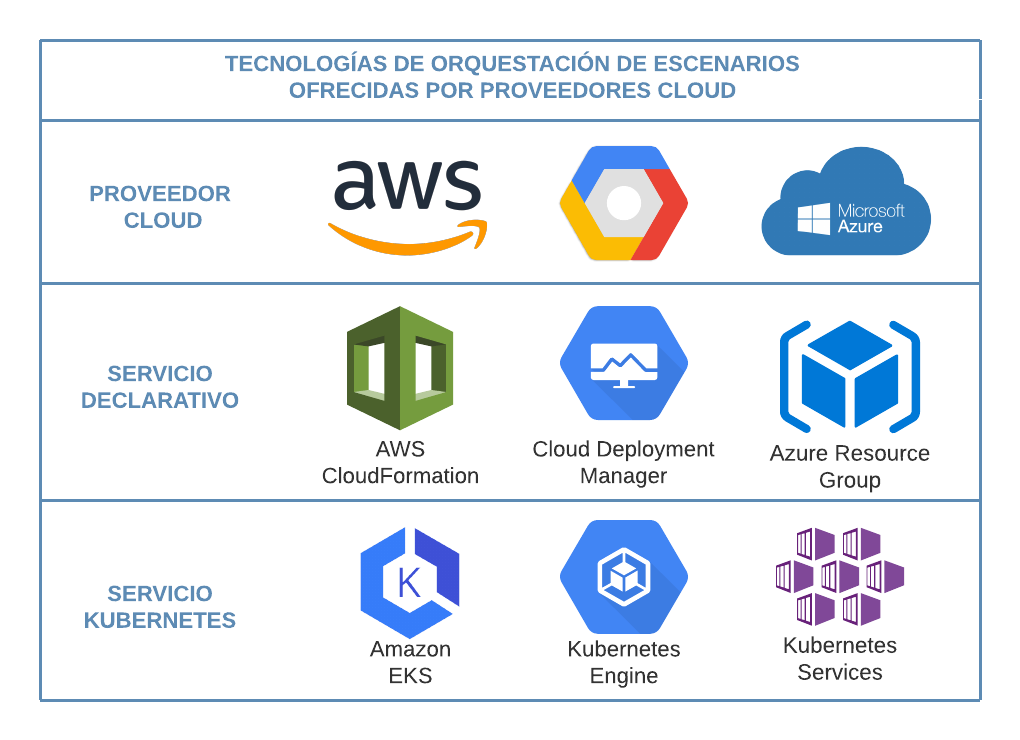
\includegraphics[width=0.8\textwidth]{../imgs/EdA/cloud/Cloud-providers.png}
% 	\caption{Tecnologías de orquestación ofrecidas por proveedores cloud}
% 	\label{fig:cloud}
% 	\end{figure}
%
% 	Estas herramientas, al estar integradas en las plataformas cloud, hacen que la orquestación de recursos en la nube sea aún más sencilla ya que se realiza la configuración a través de una interfaz gráfica muy intuitiva.
%
% 	Por otro lado, la principal desventaja que presentan radica en que su uso, al contrario que Terraform, conlleva un compromiso con el proveedor cloud que se elija. Es decir, si se decidiese usar Cloudformation de AWS, habría que tener en cuenta que esta herramienta está enfocada a la gestión de recursos exclusivamente en dicha plataforma. Por tanto, si en un momento dado se decidiese migrar a otro proveedor cloud, sería necesaria una modificación completa de todo el código, lo que implicaría una gran inversión de tiempo y recursos, ya que habría que usar otro servicio.

\section{Orquestación en Cloud} \label{sec:orqc}
    Los proveedores de nube~\cite{cloud1} permiten acceder a servicios informáticos que, de otro modo, habría que gestionar por cuenta propia, tales como infraestructura (redes, bases de datos, servidores, almacenamiento, virtualización…), plataformas (sistemas operativos, middleware o entornos de ejecución) o software como aplicaciones estándares o personalizadas que ofrecen los proveedores de servicios independientes.

\subsection{Google Cloud}
    Cuando hablamos de Google Cloud Platform (GCP), estamos ante todas las herramientas de Google disponibles en la nube que hasta ahora se ofrecían por separado. Este conjunto de servicios ofrecen prestaciones muy dispares; desde machine learning hasta Inteligencia artificial pasando por el big data, todo englobado bajo el paraguas del cloud computing.

    \begin{figure}[h]
    \centering
    
\includegraphics[width=0.4\textwidth]{../imgs/EdA/gcloud-logo.png}
    \caption{Logo de Google Cloud}
    \label{fig:gcloud}
    \end{figure}

    A la hora de desplegar escenarios de red virtualizados en la nube, de todos los servicios que ofrece Google Cloud los que más nos interesan son los relacionados con Computing y Networking. De entre estos, los más interesantes se detallan a continuación:

\subsubsection{Compute Engine}
    Compute Engine~\cite{cloud2} es un servicio de hosting y procesamiento que permite crear y ejecutar máquinas virtuales (también llamadas instancias) en la infraestructura de Google. Las instancias de Compute Engine pueden ejecutar las imágenes públicas de Linux y Windows Server que proporciona Google, así como imágenes personalizadas privadas que es posible crear o importar desde sistemas existentes. También pueden implementar contenedores de Docker.

    Cada interfaz de red de una instancia de Compute Engine está asociada con una subred de una red de VPC única y debe tener una dirección IPv4 interna principal. Una instancia puede comunicarse con instancias en la misma red de nube privada virtual (VPC) mediante la dirección IP interna de la VM. Para la comunicación con Internet, se puede usar una dirección IP externa configurada en la instancia, pero hay que tener en cuenta que de esta forma la instancia quedaría expuesta a Internet. Si no se configura ninguna dirección externa en la instancia, se puede usar Cloud NAT, que permite que ciertos recursos sin direcciones IP externas creen conexiones salientes a Internet. Los recursos externos no pueden acceder directamente a ninguna de las instancias privadas ubicadas tras la pasarela de Cloud NAT, lo que contribuye a que las VPC de Google Cloud permanezcan aisladas y protegidas.

    Una etiqueta o tag es un string de caracteres que se agrega al campo de etiquetas en un recurso, como puede ser una VM. Las etiquetas permiten hacer que las reglas de firewall y las rutas se puedan aplicar a instancias de VM específicas. Una etiqueta de red solo se aplica a las Redes de VPC que se adjuntan directamente a las interfaces de red de la instancia. Es decir, en el caso de conectar dos VPC entre sí, cada VPC solo podrá ver las etiquetas de las VM cuya interfaz de red está asociada a ella. Por lo tanto, en las reglas de FW que limitan el tráfico entre dos VPC, no se puede usar como origen o destino una etiqueta de red, ya que las VPC intercambian las rutas pero no las etiquetas. En ese caso, lo mejor es usar las direcciones IP para aplicar las reglas de FW o rutas a VM específicas.

\subsubsection{VPC}
    La nube privada virtual (VPC)~\cite{cloud3} de Google Cloud ofrece funcionalidad de red a las instancias de máquinas virtuales (VM) de Compute Engine. Una red de VPC es como una red física que se virtualiza dentro de Google Cloud, compuesta por una lista de subredes virtuales regionales (subredes) en centros de datos, todas conectadas por una red de área extensa global. Las redes de VPC están aisladas de forma lógica unas de otras dentro de Google Cloud.

    Cada red de VPC funciona como un firewall virtual distribuido. Las reglas de firewall permiten controlar qué paquetes pueden trasladarse a qué destinos. Cada red de VPC tiene dos reglas de firewall implícitas que bloquean todas las conexiones entrantes y permiten todas las conexiones salientes. Aunque las reglas de firewall se definen a nivel de red, las conexiones se permiten o deniegan por instancia, lo que permite restringir el intercambio de tráfico en función de la IP o de la etiqueta de una VM. Cada regla de firewall se aplica a la conexión entrante o saliente, pero no a ambas, y permite especificar origen, destino, protocolo, puertos y acción (permitir o denegar). Cuando se permite una conexión a través del firewall en cualquier dirección, también se permite el tráfico de retorno que coincide con esta conexión.

    También es posible definir rutas. Las rutas indican a las instancias de VM y a la red de VPC cómo enviar el tráfico de una instancia a un destino, ya sea dentro de la red o fuera de Google Cloud. Las redes de VPC incluyen algunas rutas generadas por el sistema para enrutar el tráfico entre sus subredes y enviarlo de las instancias aptas a Internet.

    Se pueden conectar dos VPC entre sí. Con el intercambio de tráfico entre redes de VPC, todas las comunicaciones se realizan mediante direcciones IP internas. Según las reglas de firewall, las instancias de VM en cada red de intercambio de tráfico pueden comunicarse entre sí sin usar direcciones IP externas. Cabe destacar que solo las redes de intercambio de tráfico directo pueden comunicarse, no se admite el intercambio de tráfico transitivo. En otras palabras, si la red de VPC N1 intercambia tráfico con las redes N2 y N3, pero estas no están conectadas directamente, la red de VPC N2 no se podrá comunicar con la N3 mediante el intercambio de tráfico entre redes de VPC. Al conectar dos VPC, las reglas de firewall (recordemos que una regla de FW se aplica a nivel de VPC) no se intercambian entre ellas. Además, como ya se ha mencionado, no es posible hacer referencia desde una VPC a etiquetas de la otra, ya que estas tampoco se intercambian.

